\documentclass[aspectratio=169]{beamer}
\usepackage{fontspec}
\usepackage{graphicx}
\usepackage{tikz}
\usepackage{xcolor}
\usetikzlibrary{calc}  

% Define custom color
\definecolor{vyperblack}{HTML}{180C25}
\definecolor{vyperviolet}{HTML}{9F4CF2}
\definecolor{vyperblue}{HTML}{75FBFB}
\definecolor{vyperyellow}{HTML}{E7FF54}
\definecolor{vyperlightgreen}{HTML}{69FF48}
\definecolor{vypergreen}{HTML}{75FBB4}
\definecolor{vyperorange}{HTML}{FFA800}
\definecolor{bubblecolor}{HTML}{DDCEAF}
\definecolor{numbertextcolor}{HTML}{FDFCFB}
\definecolor{vyperblue}{RGB}{0,0,255}
\definecolor{vypergreen}{RGB}{0,128,0}
\definecolor{vyperred}{RGB}{198,0,0}
\definecolor{vypergray}{RGB}{128,128,128}


% Set Inconsolata as the main font and for all text elements
\setmainfont{Inconsolata}[
Path = /usr/share/fonts/TTF/,
Extension = .ttf,
UprightFont = *-Regular,
BoldFont = *-Bold,
ItalicFont = *-Regular,
BoldItalicFont = *-Bold
]
\setsansfont{Inconsolata}[
Path = /usr/share/fonts/TTF/,
Extension = .ttf,
UprightFont = *-Regular,
BoldFont = *-Bold,
ItalicFont = *-Regular,
BoldItalicFont = *-Bold
]

% Set SemiExpanded Bold for titles
\newfontfamily\titlefont{Inconsolata}[
Path = /usr/share/fonts/TTF/,
Extension = .ttf,
UprightFont = *_SemiExpanded-Bold,
BoldFont = *_SemiExpanded-Bold,
ItalicFont = *_SemiExpanded-Bold,
BoldItalicFont = *_SemiExpanded-Bold
]

% Set theme
\usetheme{default}
\usecolortheme{default}

% Remove navigation symbols
\setbeamertemplate{navigation symbols}{}

% Custom background
\setbeamertemplate{background}{
	\includegraphics[width=\paperwidth,height=\paperheight]{assets/supergraphic.png}
}

\setbeamertemplate{frametitle}{
	\begin{tikzpicture}[remember picture,overlay]
		\node[anchor=north west,yshift=-10pt,xshift=10pt] at (current page.north west) {
			\includegraphics[width=0.04\textwidth]{assets/VYPER_SYMBOL_COLOR.png}
		};
		\node[anchor=north west,yshift=-10pt,xshift=0.11\textwidth] at (current page.north west) {
			\parbox{0.94\textwidth}{\raggedright\fontsize{24}{26}\titlefont\textcolor{vyperblack}{\textbf{\insertframetitle}}}
		};
	\end{tikzpicture}
}

% Custom title page
\setbeamertemplate{title page}{
	\begin{tikzpicture}[remember picture,overlay]
		\node[anchor=north west,yshift=-20pt,xshift=20pt] at (current page.north west) {
			\includegraphics[width=0.25\textwidth]{assets/vyper-logo-landscape-color-pos.pdf}
		};
		\node[anchor=north west,yshift=-40pt,xshift=20pt] at (current page.north west) {
			\parbox{0.95\textwidth}{\vspace{1.25cm}\raggedright\fontsize{32}{38}\selectfont\titlefont\textcolor{vyperblack}{\textbf{\inserttitle}}}
		};
		\node[anchor=south east,yshift=20pt,xshift=-140pt] at (current page.south east) {
			\includegraphics[width=0.2\textwidth]{assets/avatar.png}
		};
		\node[anchor=south east,yshift=45pt,xshift=-80pt] at (current page.south east) {
			\fontsize{24}{28}\selectfont\textcolor{vyperblack}{\textbf{benny}}
		};
		\node[anchor=south east,yshift=30pt,xshift=-10pt] at (current page.south east) {
			\fontsize{18}{22}\selectfont\textcolor{vyperblack}{\small{Developer Advocate - Vyper}}
		};
		\node[anchor=south east,yshift=18pt,xshift=-65pt] at (current page.south east) {
		\fontsize{18}{22}\selectfont\textcolor{vyperblack}{\small{ETH Riyadh 2024}}
		};
		
	\end{tikzpicture}
}

% Set all text to vyperblack
\setbeamercolor{normal text}{fg=vyperblack}
\setbeamercolor{frametitle}{fg=vyperblack}
\setbeamercolor{title}{fg=vyperblack}

\title{Onboarding the next generation of web3 developers}

\begin{document}
	
	% Title slide
	\begin{frame}[plain]
		\titlepage
	\end{frame}
	
		% What's Vyper? slide
\begin{frame}
	\frametitle{What's Vyper?}
	
	\begin{itemize}
		\item A Pythonic smart contract programming language for the EVM
		\item Designed for simplicity, safety and efficiency
		\item Used by major protocols across the Ethereum ecosystem
	\end{itemize}
	
	\vspace{0.75cm} % Adjust this value to control space before the logos
	
	\begin{tikzpicture}[remember picture,overlay]
		\foreach \x/\name in {0/Curve, 1/Frax, 2/Lido, 3/{Perpetual Protocol}, 4/Velodrome, 5/Yearn, 6/{Ripe Finance}}
		{
			\node[anchor=north] at ($(current page.north)+(-0.35\paperwidth+0.10\paperwidth*\x,-0.57\paperheight)$) {
				\includegraphics[width=0.06\paperwidth]{assets/\name.png}
			};
			\node[anchor=north, text width=0.12\paperwidth, align=center] at ($(current page.north)+(-0.35\paperwidth+0.10\paperwidth*\x,-0.71\paperheight)$) {
				\footnotesize\name
			};
		}
	\end{tikzpicture}
\end{frame}

	\begin{frame}
		\frametitle{What's Vyper?}
		
		\begin{itemize}
			\item Vyper is currently the second most popular smart contract language in the Ethereum ecosystem, after Solidity
			\vspace{0.5em}
			\item Vyper is positioning itself to be the first choice for all new web3 developers:
			\begin{itemize}
				\item Vyper is easy, safe and efficient by default
				\item You don't need to be an EVM wizard to write good, optimized contracts
			\end{itemize}
		\end{itemize}
		
	\end{frame}
	
	
\begin{frame}
	\frametitle{Web3 Developer Landscape}
	
	\vspace{2.5em}
	\begin{columns}[T]
		\begin{column}{0.4\textwidth}
			\includegraphics[width=\columnwidth, height=0.8\textheight]{charts/developers.png}
		\end{column}
		
		\begin{column}{0.55\textwidth}
			\begin{itemize}
				\item There are less than 30,000 active developers accross the industry, less than in many individual tech companies
				\vspace{1em}
				\item New developers are the largest share of all Web3 developers
				\vspace{1em}
				\item As the industry continues to grow, we will see influxes of new developers - both new graduates and experienced engineers
			\end{itemize}
		\end{column}
	\end{columns}
	
\end{frame}
	

\begin{frame}
	\frametitle{Vyper is Beginner Friendly}
	\begin{columns}[T,totalwidth=\textwidth]
		\begin{column}{0.35\textwidth}
			\vspace{2em} % More space below title
			\includegraphics[width=\columnwidth,height=0.75\paperheight,keepaspectratio]{charts/favoritelanguage.png}
		\end{column}
		\begin{column}{0.65\textwidth}
			\vspace{2em} % More space below title
			\setbeamercolor{itemize item}{fg=vyperviolet}
			\setbeamercolor{itemize subitem}{fg=vyperviolet}
			\setbeamercolor{itemize subsubitem}{fg=vyperviolet}
			\begin{itemize}
				\item \textbf{Vyper's syntax is very similar to Python}, a language that most developers are not only familiar with but \textbf{want} to work with\\
			\end{itemize}
			
			\vspace{3em} % Space before the code bubble
			
			\begin{tikzpicture}[remember picture,overlay]
				\node[anchor=north west, 
				fill=bubblecolor!70, 
				opacity=0.5,
				rounded corners, 
				text width=0.54\paperwidth,
				inner sep=10pt,
				minimum height=7em] 
				at ($(current page.north west)+(0.37\paperwidth,-0.45\paperheight)$) 
				(codebubble) {};
				
				\node[anchor=north west, 
				font=\footnotesize\ttfamily, 
				text width=0.52\paperwidth] 
				at ($(codebubble.north west)+(0.5em,-0.5em)$) 
				{
					\textcolor{vyperviolet}{@external}\\
					\textcolor{vyperblack}{def} \textcolor{vyperviolet}{hello\_year}\textcolor{vyperblack}{() ->} \textcolor{vyperviolet}{uint256}\textcolor{vyperblack}{:}\\
					\hspace{1em}\textcolor{vyperblack}{print(}\textcolor{vyperviolet}{"Hello, World!"}\textcolor{vyperblack}{)}\\
					\hspace{1em}\textcolor{vyperblack}{return} \textcolor{vyperviolet}{2024}
				};
			\end{tikzpicture}
		\end{column}
	\end{columns}
\end{frame}



\begin{frame}
	\frametitle{Vyper is Safe by Default}
	\begin{columns}[T,totalwidth=\textwidth]
		\begin{column}{0.35\textwidth}
			\vspace{2em} % More space below title
			\includegraphics[width=\columnwidth,height=0.75\paperheight,keepaspectratio]{charts/security.png}
		\end{column}
		\begin{column}{0.65\textwidth}
			\vspace{2em} % More space below title
			\setbeamercolor{itemize item}{fg=vyperviolet}
			\setbeamercolor{itemize subitem}{fg=vyperviolet}
			\setbeamercolor{itemize subsubitem}{fg=vyperviolet}
			\begin{itemize}
				\item \textbf{No footguns}: Safe arithmetic, no operator or function overloading, no modifiers\\
				\item \textbf{Modularity over inheritance}: Inheritance is hard to read, hard to audit and has led to multiple exploits\\
				\item \textbf{Fixed gas limits}: Finite length loops and no recursive calls prevent gas limit attacks.
				\item \textbf{No assembly}: Low level attempts at optimization are another common source of vulnerabilities\\
			\end{itemize}
			
		\end{column}
	\end{columns}
\end{frame}



\begin{frame}
	\frametitle{Vyper is Optimal by Default}
	\begin{columns}[T,totalwidth=\textwidth]
		\begin{column}{0.35\textwidth}
			\vspace{2em} % More space below title
			\includegraphics[width=\columnwidth,height=0.75\paperheight,keepaspectratio]{charts/gaserc20.png}
		\end{column}
		\begin{column}{0.65\textwidth}
			\vspace{2em} % More space below title
			\setbeamercolor{itemize item}{fg=vyperviolet}
			\setbeamercolor{itemize subitem}{fg=vyperviolet}
			\setbeamercolor{itemize subsubitem}{fg=vyperviolet}
			\begin{itemize}
				\item Vyper contracts have \textbf{lower gas usage} and up to \textbf{50\% lower bytecode size} compared to Solidity\\
				\item Optimizations are done directly by the compiler. There is no need for tricks and hacks to get optimal efficiency.\\
				\item This makes for contracts that are \textbf{easier to write and easier to read}\\
			\end{itemize}
			
		\end{column}
	\end{columns}
\end{frame}

\begin{frame}
	\frametitle{Vyper is Optimal by Default}
	
	\begin{tikzpicture}[remember picture,overlay]
		% First box (left)
		\node[anchor=north west, 
		fill=bubblecolor!70, 
		opacity=0.5,
		rounded corners, 
		text width=0.4\paperwidth,
		inner sep=10pt,
		minimum height=12em] 
		at ($(current page.north west)+(0.03\paperwidth,-0.25\paperheight)$) 
		(box1) {};
		
		\node[anchor=north west, 
		font=\tiny\ttfamily, 
		text width=0.4\paperwidth] 
		at ($(box1.north west)+(0.5em,-0.5em)$) 
		{
			\textcolor{vyperviolet}{assembly} \{\\
			\hspace{0.5em}\textcolor{vyperblue}{let} from\_ := \textcolor{vypergreen}{shl}(96, from)\\
			\hspace{0.5em}\textcolor{vypergreen}{mstore}(0x0c, \textcolor{vypergreen}{or}(from\_, \_BALANCE\_SLOT\_SEED))\\
			\hspace{0.5em}\textcolor{vyperblue}{let} fromBalanceSlot := \textcolor{vypergreen}{keccak256}(0x0c, 0x20)\\
			\hspace{0.5em}\textcolor{vyperblue}{let} fromBalance := \textcolor{vypergreen}{sload}(fromBalanceSlot)\\
			\hspace{0.5em}\textcolor{vyperviolet}{if} \textcolor{vypergreen}{gt}(amount, fromBalance) \{\\
			\hspace{1em}\textcolor{vypergreen}{mstore}(0x00, 0xf4d678b8) \textcolor{vypergray}{// `InsufficientBalance()`.}\\
			\hspace{1em}\textcolor{vypergreen}{revert}(0x1c, 0x04)\\
			\hspace{0.5em}\}\\
			\hspace{0.5em}\textcolor{vypergreen}{sstore}(fromBalanceSlot, \textcolor{vypergreen}{sub}(fromBalance, amount))\\
			\hspace{0.5em}\textcolor{vypergreen}{mstore}(0x00, to)\\
			\hspace{0.5em}\textcolor{vyperblue}{let} toBalanceSlot := \textcolor{vypergreen}{keccak256}(0x0c, 0x20)\\
			\hspace{0.5em}\textcolor{vypergreen}{sstore}(toBalanceSlot, \textcolor{vypergreen}{add}(\textcolor{vypergreen}{sload}(toBalanceSlot), amount))\\
			\hspace{0.5em}\textcolor{vypergreen}{mstore}(0x20, amount)\\
			\hspace{0.5em}...\\
			\}
		};
		
		% Second box (right)
		\node[anchor=north east, 
		fill=bubblecolor!70, 
		opacity=0.5,
		rounded corners, 
		text width=0.4\paperwidth,
		inner sep=10pt,
		minimum height=12em] 
		at ($(current page.north east)+(-0.03\paperwidth,-0.25\paperheight)$) 
		(box2) {};
		
		\node[anchor=north west, 
		font=\tiny\ttfamily, 
		text width=0.43\paperwidth] 
		at ($(box2.north west)+(0.5em,-0.5em)$) 
		{
			\textcolor{vyperblue}{self}.\_before\_token\_transfer(owner, to, amount)\\
			\\
			owner\_balanceOf: \textcolor{vyperviolet}{uint256} = \textcolor{vyperblue}{self}.balanceOf[owner]\\
			\textcolor{vyperviolet}{assert} (owner\_balanceOf >= amount,\\ \textcolor{vypergreen}{"erc20: transfer amount exceeds balance")}\\\newline
			\textcolor{vyperblue}{self}.balanceOf[owner] = unsafe\_sub(owner\_balanceOf, amount)\\
			\textcolor{vyperblue}{self}.balanceOf[to] = unsafe\_add(\textcolor{vyperblue}{self}.balanceOf[to], amount)\\
			\\
			\textcolor{vyperviolet}{log}  IERC20.Transfer(sender=owner, receiver=to, value=amount)\\
			\\
			\textcolor{vyperblue}{self}.\_after\_token\_transfer(owner, to, amount)
			\\...
		};
		
		% Solady label
		\node[anchor=south, font=\small] 
		at ($(box1.south)+(0,-2em)$) 
		{Solady};
		\node[anchor=north] at ($(current page.north)+(-1.25,-0.65\paperheight)$) 
		{\includegraphics[width=2cm]{assets/solidity.png}};
		
		% Snekmate label
		\node[anchor=south, font=\small] 
		at ($(box2.south)+(0,-2em)$) 
		{Snekmate};
		\node[anchor=north] at ($(current page.north)+(+0.4\paperwidth,-0.65\paperheight)$) 
		{\includegraphics[width=1cm]{assets/VYPER_SYMBOL_COLOR.png}};
	\end{tikzpicture}
\end{frame}

\begin{frame}
	\frametitle{Vyper is Optimal by Default}
	
	\begin{tikzpicture}[remember picture,overlay]
		% First box (top-left)
		\node[anchor=north west, 
		fill=bubblecolor!70, 
		opacity=0.5,
		rounded corners, 
		text width=0.35\paperwidth,
		inner sep=10pt,
		minimum height=7em] 
		at ($(current page.north west)+(0.03\paperwidth,-0.25\paperheight)$) 
		(box1) {};
		
		\node[anchor=north west, 
		font=\footnotesize\ttfamily, 
		text width=0.38\paperwidth] 
		at ($(box1.north west)+(0.5em,-0.5em)$) 
		{
			\textcolor{vyperviolet}{@external}\\
			\textcolor{vyperviolet}{def} \textcolor{vyperblack}{get\_six() ->} \textcolor{vyperviolet}{uint256}\textcolor{vyperblack}{:}\\
			\hspace{1em}\textcolor{vyperblack}{a:} \textcolor{vyperviolet}{uint256} \textcolor{vyperblack}{= 3}\\
			\hspace{1em}\textcolor{vyperblack}{b:} \textcolor{vyperviolet}{uint256} \textcolor{vyperblack}{= 2}\\
			\hspace{1em}\textcolor{vyperblack}{return a * b}
		};
		
		% Second box (top-right)
		\node[anchor=north west, 
		fill=bubblecolor!70, 
		opacity=0.5,
		rounded corners, 
		text width=0.35\paperwidth,
		inner sep=10pt,
		minimum height=7em] 
		at ($(current page.north west)+(0.57\paperwidth,-0.25\paperheight)$) 
		(box2) {};
		
		\node[anchor=north west, 
		font=\footnotesize\ttfamily, 
		text width=0.38\paperwidth] 
		at ($(box2.north west)+(0.5em,-0.5em)$) 
		{
			\textcolor{vyperviolet}{@external}\\
			\textcolor{vyperviolet}{def} \textcolor{vyperblack}{get\_six() ->} \textcolor{vyperviolet}{uint256}\textcolor{vyperblack}{:}\\
			\hspace{1em}\textcolor{vyperblack}{return 6}
		};
		
		% Third box (bottom-left)
		\node[anchor=north west, 
		fill=bubblecolor!70, 
		opacity=0.5,
		rounded corners, 
		text width=0.35\paperwidth,
		inner sep=10pt,
		minimum height=7em] 
		at ($(current page.north west)+(0.03\paperwidth,-0.65\paperheight)$) 
		(box3) {};
		
		\node[anchor=north west, 
		font=\footnotesize\ttfamily, 
		text width=0.38\paperwidth] 
		at ($(box3.north west)+(0.5em,-0.5em)$) 
		{
			\textcolor{vyperviolet}{function} \textcolor{vyperblack}{get\_six()} \\
			\textcolor{vyperviolet}{public pure returns} \textcolor{vyperblack}{(uint256) \{}\\
			\hspace{1em}\textcolor{vyperviolet}{uint256} \textcolor{vyperblack}{a = 3;}\\
			\hspace{1em}\textcolor{vyperviolet}{uint256} \textcolor{vyperblack}{b = 2;}\\
			\hspace{1em}\textcolor{vyperblack}{return a * b;}\\
			\textcolor{vyperblack}{\}}
		};
		
		% Fourth box (bottom-right)
		\node[anchor=north west, 
		fill=bubblecolor!70, 
		opacity=0.5,
		rounded corners, 
		text width=0.35\paperwidth,
		inner sep=10pt,
		minimum height=7em] 
		at ($(current page.north west)+(0.57\paperwidth,-0.65\paperheight)$) 
		(box4) {};
		
		\node[anchor=north west, 
		font=\footnotesize\ttfamily, 
		text width=0.38\paperwidth] 
		at ($(box4.north west)+(0.5em,-0.5em)$) 
		{
			\textcolor{vyperviolet}{function} \textcolor{vyperblack}{get\_six()} \\
			\textcolor{vyperviolet}{public pure returns} \textcolor{vyperblack}{(uint256) \{}\\
			\hspace{1em}\textcolor{vyperblack}{return 6;}\\
			\textcolor{vyperblack}{\}}
		};
		
		% Vyper symbol and text
		\node[anchor=north] at ($(current page.north)+(0,-0.27\paperheight)$) 
		{\includegraphics[width=1cm]{assets/VYPER_SYMBOL_COLOR.png}};
		\node[anchor=north, text width=2cm, align=center] 
		at ($(current page.north)+(0,-0.42\paperheight)$) 
		{\textcolor{vypergreen}{Equivalent in Vyper}};
		
		% Solidity symbol and text
		\node[anchor=north] at ($(current page.north)+(0,-0.65\paperheight)$) 
		{\includegraphics[width=2cm]{assets/solidity.png}};
		\node[anchor=north, text width=2.2cm, align=center] 
		at ($(current page.north)+(0,-0.82\paperheight)$) 
		{\textcolor{vyperred}{Different in Solidity}};
	\end{tikzpicture}
\end{frame}


\begin{frame}
	\frametitle{Vyper is Readable}
	
	\begin{columns}[T,totalwidth=\textwidth]
		\begin{column}{0.4\textwidth}
			\centering
			\includegraphics[width=\textwidth]{assets/stacktoodeep.png}
		\end{column}
		
		\begin{column}{0.55\textwidth}
			\begin{itemize}
				\item \textbf{No stack too deep errors} forcing rewrites that impede readability
				\vspace{1em}
				\item \textbf{Faster, easier and cheaper} to audit
			\end{itemize}
		\end{column}
	\end{columns}
\end{frame}

\begin{frame}
	\frametitle{Vyper is for Everyone}
	
	
	\vspace{2em}
	
	\begin{itemize}
		\item Vyper is easy to use, easy to set up: 
		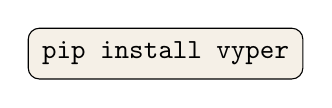
\begin{tikzpicture}[baseline]
			\node[draw, fill=bubblecolor!30, rounded corners, inner sep=5pt] 
			{\texttt{pip install vyper}};
		\end{tikzpicture}
		
		\item You don't have to start with custodial contracts: util contracts for analytics, zaps for DeFi, simple on-chain games are all great to get started.
	\end{itemize}
	
	\begin{center}
		\begin{tabular}{@{}c@{\hspace{3em}}c@{\hspace{3em}}c@{}}
			\includegraphics[width=0.25\textwidth]{assets/qrtg.png} &
			\includegraphics[width=0.25\textwidth]{assets/qrdiscord.png} &
			\includegraphics[width=0.25\textwidth]{assets/qrcyfrin.png} \\
			Telegram Channel & Discord Server & Cyfrin Course
		\end{tabular}
	\end{center}
\end{frame}

\end{document}